%===============
%一行目に必ず必要
%文章の形式を定義
%===============
\documentclass{ujarticle}
%===============
%パッケージの定義、必要か不明
%===============
%この下4つを加えることで、mathbbが機能した
\usepackage{amsthm}
\usepackage{amsmath}
\usepackage{amssymb}
\usepackage{amsfonts}
\usepackage{my-default}
%リンク用パッケージ
\usepackage[dvipdfmx]{hyperref}
%tikz用パッケージ
\usepackage[dvipdfmx]{graphicx}
\usepackage{tikz}
\usepackage{tikz-cd}
\usepackage{my-default}

%複数行コメント
%\usepackage{comment}

%修論当時
\newcommand\X{\mathfrak{X}}
\newcommand\p{\mathfrak{p}}
\newcommand\f{\mathfrak{f}}
\newcommand\m{\mathfrak{m}}
\newcommand\G{\mathrm{Gal}}
\newcommand\iy{\infty}
\def\F{F_{\infty}}
\def\M{M_{\infty}}
\def\bgn{\begin}
\def\c{c_{F_{\iy}/M_{\iy}}}
\def\n{\nu_{F_{\iy}/M_{\iy}}}

\newcommand\bqy{\bgn{eqnarray*}}
\newcommand\eqy{\end{eqnarray*}}
\newcommand\mac{\mathcal}
\newcommand\mf{\mathfrak}
\newcommand\mr{\mathrm}
\newcommand\mb{\mathbb}

\newcommand\vp{\varprojlim}
\newcommand\ot{\otimes}


\renewenvironment{itemize}%
{%
   \begin{list}{\parbox{1zw}{$\bullet$}}% 見出し記号/直後の空白を調節
   {%
      \setlength{\topsep}{0zh}
      \setlength{\itemindent}{0zw}
      \setlength{\leftmargin}{2zw}%  左のインデント
      \setlength{\rightmargin}{0zw}% 右のインデント
      \setlength{\labelsep}{1zw}%    黒丸と説明文の間
      \setlength{\labelwidth}{3zw}%  ラベルの幅
      \setlength{\itemsep}{0em}%     項目ごとの改行幅
      \setlength{\parsep}{0em}%      段落での改行幅
      \setlength{\listparindent}{0zw}% 段落での一字下り
   }
}{%
   \end{list}%
}


\renewenvironment{enumerate}
{
\begin{list}{\arabic{enumi}.}
{
\usecounter{enumi}
\setlength{\topsep}{0zh}
\setlength{\itemindent}{0zw}
\setlength{\leftmargin}{2zw} % 左のインデント
\setlength{\rightmargin}{0zw} % 右のインデント
\setlength{\labelsep}{1zw} % 黒丸と説明文の間
\setlength{\labelwidth}{3zw} % ラベルの幅
\setlength{\itemsep}{0em} % 項目ごとの改行幅
\setlength{\parsep}{0em} % 段落での改行幅
\setlength{\listparindent}{1zw} % 段落での一字下り
}
}{
\end{list}
}



%タイトルデータ
\title{TESTING THE MANIFOLD HYPOTHESIS}
\author{test}
\date{2017/01/29}
%===============
%定理環境の設定
%セクション毎
%===============


%この論文紹介用定義
\newcommand{\bh}[2]{B_{\mathcal{H}}(#1,#2)}
\newcommand{\bpa}{B_{\Pi_1}(0,r)}
\newcommand{\bpb}{B_{\Pi_2}(0,r)}
\newcommand{\bpd}{B_{\Pi}(0,r)}
\newcommand{\bp}[3]{B_{\Pi_{#3}}(#1,#2)}
\newcommand{\gn}[4]{||\Gamma_{#1}||_{C^{1,1}(\bp{#2}{#3}{#4})}}
\newcommand{\gnaaad}{||\Gamma_1||_{C^{1,1}(\bp{z_1}{r_1}{})}}
\newcommand{\gnd}{||\Gamma||_{C^{1,1}(\bpd)}}
\newcommand{\gdvt}{\mathcal{G}(d,V,\tau)}
\newcommand{\Me}{M_{erm}}
\newcommand{\Px}{\Pi_x}
\newcommand{\Py}{\Pi_y}


\begin{document}
\section{Introduction}
\label{sec:Introduction}
岩澤理論と自分の修士論文を話したい.

前半は岩澤理論の基本的な話をする.
最低限の準備が終われば,今回の主結果の一つについて記載する.
後半にはFitting Idealの話を書く.
\section{Bernouli number and zeta function}
\label{sec:Bernouli number and zeta function}
\subsection{Bernouli number}
\label{sub:Bernouli number}
ベルヌーイ数を定義する.
\begin{dfn}
 ベルヌーイ数$B_n$を以下で定義する.
 \begin{equation*}
  \sum_{n=0}^k B_n \binom{k+1}{n}=k+1
 \end{equation*}
\end{dfn}

指標を定義する.
$\xi$

\section{Algebra and Cyclotomic Fields}
\label{sec:Algebra and Cyclotomic Fields}
円分体とp進体に関する代数的な話を記述する

\subsection{p-adic Weirstarss Thorem}
\label{sub:p-adic Weirstarss Theorem}

\subsection{Kummer Congurence}
\label{sub:Kummer Congurence}

\subsection{Leopold Conjecture}
\label{sub:Leopold Conjecture}



\section{p-adic L function}
\label{sec:p-adic L function}


\subsection{Mahler Theorem}
\label{sec:Mahler Theorem}

\subsection{Construction of p-adic L function}
\label{sub:Construction of p-adic L function}
$H(S,a,F)$を以下で定義する.
\begin{equation*}
 H(S,a,F)=\sum_{m \equiv a \mbox{mod}F,m >0}m^{-s}=\sum_{n=0}^{\infty}\frac{1}{(a+nF)^s}
       =F^{-s} \zeta(s,\frac{a}{F})
\end{equation*}
ここで,$s \in \mathbb{C},a,F \in \mathbb{Z}$で$0 < a< F$を満たす.
\begin{equation*}
  \zeta(s,b)=\sum_{n=0}^{\infty}\frac{1}{(n+b)^s}
\end{equation*}
はHurwitz zeta functionである.
この時,
以下が成り立つ.


\subsection{StickelBelger Theorem}
\label{sub:StickelBelger Theorem}


\subsection{Measure and Distribution}
\label{sub:Measure and Distribution}


\section{Euler System}
\label{sec:Euler System}

\subsection{definiton of Euler Ssytem}
\label{sub:definiton of Euler Ssytem}

\subsection{Cyclotomic units}
\label{sub:Cyclotomic units}

\subsection{Vandiver's Conjecture}
\label{sub:Vandiver's Conjecture}


\subsection{Elliptic units}
\label{sub:Elliptic units}

\section{The Second Case of Fermat's Last Theorem}
\label{sec:The Second Case of Fermat's Last Theorem}

\section{Iwasawa theory }
\label{sec:Iwasawa theory }



\section{Fitting Ideal}
\label{sec:FItting Ideal}
岩澤理論の精密化ではCharacateristic Idealではなく,Fitting Idealを調べる.
ここでは,Fitting Idealの基本的な定義と性質をみる.
Fitting Idealが岩澤理論で使われる理由として以下の二点を示す.
\begin{itemize}
  \item $\Lambda$加群$M$に対し,$Char(M) \subset Fitt_0(M)$
  \item $\Lambda$加群$M,N$がpseudo-isoの時,$Fitt_i(M)=Fitt_i(N)$となる.
\end{itemize}

Fitting IdealはPID上の有限生成加群の理論(単因子論)を一般化した理論である.
Fitting Idealはfinitely presented moduleを用いて定義されるため,finitely presentedを定義する.
\begin{dfn}
環$R$に対し,$M$がfintely presented $R$-moduleとは,
\begin{equation*}
 \phi: R^m \twoheadrightarrow M
\end{equation*}
であって,$\ker \phi$が$R$-moduleとして有限生成である$\phi$が存在すること.
すまわち,
\begin{equation*}
 R^n \to R^m \xrightarrow{\phi} M \to 0
\end{equation*}
がexactであること.
\end{dfn}

\begin{epl}
 $R=\mathbb{Q}[X_1 ,\dots,X_n,\dots]$とする.$M$を$(X_1)$とし,$\phi$を自然な射影とすると
  $\ker \phi=(X_2,\dots X_n \dots)$となり,これは有限生成ではない.もし有限生成だとすると,
  生成元によって,任意の$X_i$を書くことができ,矛盾する.
\end{epl}

\begin{rem}
   それがなぜ矛盾かをきちんと書こうとすると難しい.
\end{rem}

\begin{lem}
 $R$がネータなら,finitely generetatedとfinitely presentedは同値
\end{lem}
\begin{proof}
 $R$がNeotherなので,$R^m$もNeotherになる.(昇鎖の停止から確認すればよい.)
 これより$\ker \phi$はNeother環のイデアルとなるので,$R^m$加群として有限生成となり,$R$加群としても有限生成となる.
\end{proof}

Fitting Idealを定義する.
\begin{dfn}
  \begin{equation*}
   R^n \xrightarrow{f} R^m  \to M \to 0
  \end{equation*}
がexactである時,$f$の表現行列を$A$とする.
$A$の$n-i \times n-i$小行列の行列式全体で生成されるイデアルを$Fitt_iR$と書く.
また,$i \ge n$の時,$Fitt_iR=R$とする.
\end{dfn}

\begin{epl}
 $R$をPIDとし,$M$を有限生成Torsion加群とする.この時,
  単因子論より$M \simeq \oplus_{i=1}^n R/e_i (e_i | e_{i+1})$となる.
  この時,$Fitt_i(R)=(e_1 \cdots e_i)$となる.
\end{epl}


\begin{prop}
 $R$を環,$M$をfinitely presented $R$-moduleとする.
 この時,$Fitt_i(M) \otimes R_{\mathfrak{p}} \simeq  Fitt_i(R_{\mathfrak{p}})M_{\mathfrak{p}}$
\end{prop}

\begin{proof}
以下の可換図式は,行が完全なため,上の行と下の行からFitting Idealの生成元は上と下で一致する.


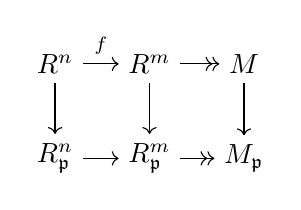
\begin{tikzpicture}[auto]
  \node (Rn) at (0, 1.2) {$R^n$}; \node (Rm) at (1.2, 1.2) {$R^m$};\node (M) at (2.4, 1.2) {$M$};
  \node (Rpn) at (0, 0) {$R_{\mathfrak{p}}^n$};   \node (Rpm) at (1.2, 0) {$R_{\mathfrak{p}}^m$};\node (Mp) at (2.4, 0) {$M_{\mathfrak{p}}$};
  \draw[->] (Rn) to node {$\scriptstyle f$} (Rm);\draw[->>] (Rm) to node {} (M);
  \draw[->](Rn) to node {} (Rpn);\draw[->](Rm) to node {} (Rpm);\draw[->](M) to node {} (Mp);
  \draw[->] (Rpn) to node {} (Rpm);\draw[->>] (Rpm) to node {} (Mp);
\end{tikzpicture}
よって,$Fitt_i(M)R_{\mathfrak{p}}=Fitt_i(M_{\mathfrak{p}})$となる.
また,局所化がflatなことから$Fitt_i(M)R_{\mathfrak{p}}=Fitt_i(M) \otimes R_{\mathfrak{p}}$となる.

\end{proof}

\begin{prop}
 $R$がNormalなら$R = \cap_{ \scriptscriptstyle  \mathfrak{p}, \mathrm{ht}\mathfrak{p}=1 }R_{\mathfrak{p}} $
\end{prop}
\begin{proof}
 略
\end{proof}

\begin{prop}
 $R$がNormal, $M$をfinitely presented $R$-moduleとする.
 この時,$Fitt_i(M) \otimes \cap_{\mathfrak{p},\mathrm{ht}\mathfrak{p}=1} R_{\mathfrak{p}} \simeq  \cap_{\mathfrak{p},\mathrm{ht}\mathfrak{p}=1} Fitt_i(R_{\mathfrak{p}})M_{\mathfrak{p}}$
\end{prop}
\begin{proof}
 包含は明らかなので,逆を言えばよい.逆は上と同じ議論をすることで言える.
\end{proof}

\begin{prop}
 $\mathbb{Z}_p[[T_1,\dots ,T_k]] $は正規である.
\end{prop}
以降では$\Lambda = \mathbb{Z}_p[[T_1,\dots ,T_k]] $とする.
\begin{dfn}
  有限生成$\Lambda$加群$A$がpseudo-nullとは任意のheight1の素イデアル$\mathfrak{p}$で局所化した時に
  $0$となること.
\end{dfn}

\begin{prop}
 $\mathbb{Z}_p[[T]]$加群の時は,pseudonullは位数が有限であることと同値.
\end{prop}

\begin{thm}[有限生成$\Lambda$加群の基本定理]
  略
\end{thm}

\begin{prop}
   $\Lambda$加群$M,N$がpseudo-isoの時,$Fitt_i(M)=Fitt_i(N)$となる.
\end{prop}
\begin{rem}
 なんか不安になってきた.今考えていることが正しいのならCharateristc idealとFitting Idealが真に一致しそう.

\end{rem}

\section{Iwasawa Thoery of Etale Cohomology}
\label{sec:Iwasawa Thoery of Etale Cohomology}

\section{Main Thoerem 1 of my consequence}
\label{sec:Main Thoerem 1 of my consequence}


\section{Kurihara's Lemma}
\label{sec:Kurihara's Lemma}

\section{Main Thoerem 2 of my consequences}
\label{sec:Main Thoerem 2 of my consequences}



\part{原稿メモ}
2時間を以下の予定で話したい
\begin{verbatim}
- 歴史(30分)
 0. 類体論と岩澤理論の基本完全系列
 1. 岩澤主予想の基本的な定式化とEuler System
 2. 虚二次体の場合のEuler System
 3. Euler Systemの既存の課題
 4. Johnson Kingsのアイディア
- 自分の結果,及び証明の基本的な道具紹介(30分)
 1. 結果
   - 岩澤主予想
   - 岩澤主予想のFitting Ideal版
 2. 基本的な道具
   - Johoson-Kingsの結果
   - Poitou-Tate exact sequence
   - 岩澤理論の基本完全系列
   - 実際に示す??
   - Kurihara's lemma
- 証明の詳細(60分)
\end{verbatim}

最初は上記のように考えていたが、方針を変更して発表時のレベルを分けて以下の二つとする.

\textbf{Doctor向け}
\begin{enumerate}
  \item Intro 5分
  \item Johonson Kings 5分
  \item 楕円単数とその性質について 10分
  \item 主定理1の証明 30分
  \item Kuriharaさんの結果(古典的なもの) 10分
  \item 主定理2の証明 20分
  \item 今後 10分
\end{enumerate}

\textbf{For Sunday mathmatican}
\begin{enumerate}
  \item 岩澤理論の基本 30分
  \item Johnson Kings 10分
  \item 証明の方針(1)  基本的なコホモロジーの計算 30分
  \item 最低限の道具  15分
  \item 証明の方針(1)2 拡大次数がpであるが故の難点、
  及び、$\mathfrak{p}$と$p$の違い 30分
  \item Kuriharaさんの結果について
\end{enumerate}



\section{Introduction}
\label{sec:Introduction}
岩澤理論は数論で重要な位置を占めるイデアル類群の情報を調べるために創始され,
イデアル類群の逆極限で得られる岩澤加群を理解することが岩澤理論の目的の一つである.
特に,岩澤加群が$p$進$L$関数を用いて書くことは岩澤主予想と言われ,岩澤理論の一番重要な問題となっている.
岩澤主予想は1980年代に保型形式を用いることで$\mathbb{Q}$と総実体の場合に解決された.
また,1990年代になるとEuler Systemと呼ばれる代数的な方法により,虚二次体の場合に証明された.
ただし,これは虚二次体上拡大次数が$p$で割れる時は示せておらず,完全な解決ではなかった.
この頃になると,岩澤主予想のコホモロジーによる定式化,楕円曲線の岩澤理論,モチーフの岩澤理論等様々な一般化がされ始めた
2000年代になると,Johonson,Kingsにより,虚二次体上のコホモロジーによる岩澤主予想が完全に解決された.
これを用いて,古典的な岩澤主予想を示すことがこの論文の主定理の一つである.
この論文の2つ目の主定理はFitting Idealによる岩澤主予想の精密化についてである.
Kuriharaによる論文を参考に,主定理1の結果を用いてFitting Idealによる精密化を行った.

\section{岩澤理論の基本}
\label{岩澤理論の基本}
岩澤理論を初学者のために,以下の岩澤理論の関する基本的な結果を述べる.
\begin{enumerate}
  \item 有限生成$\Lambda$加群の構造定理と岩澤類数公式
  \item 岩澤理論の基本完全系列
  \item Euler System
  \item Kubota-Leopoldの$p$進L関数
  \item 円単数,楕円単数とEuler System,$p$進L関数との関係
\end{enumerate}

\subsection{有限生成$\Lambda$加群の構造定理と岩澤類数公式}
\label{sub:有限生成}
ここでは$\Lambda$を混票数$(0,p)$の完備離散付値環であって,剰余体の位数が有限となる環係数の形式的べき級数環とする.
有限生成,$\Lambda$加群には単因子論の類似が成り立つ.
ただし単因子論は同型の変形であったが,ここではpseudo isomorphismとなる.
\begin{dfn}
  $\Lambda$加群$A$の位数が有限である時pseudo-nulという.$f:A \to B$のkernelとcokernelがpseudo-nullの時
  $A$と$B$は\textbf{pseudo isomorphic}といい,$A \sim B$とかく.
\end{dfn}



\subsection{岩澤理論の基本完全系列}
\label{sub:基本完全系列}
大域類体論より,
\begin{equation*}
   E_K \otimes \mathbb{Z}_p \to \prod_{\mathfrak{p} | p} U_{K_{\mathfrak{p}}} \to \mathrm{Gal}(H_p/K) \to \mathrm{Gal}(H/K) \to 1
\end{equation*}
が成り立つ.これの逆極限を取ったものを岩澤理論の基本完全系列と呼ぶ.
これは岩澤理論で重要な情報であるイデアル類群と代数体,局所体の単数の関係を述べたものとなり,
円単数や楕円単数で割ることにより,岩澤主予想の様々な定式化を可能とするものである.
\begin{rem}
\begin{equation*}
  E_K\otimes \mathbb{Z}_p \to \prod_{\mathfrak{p} | p} U_{K_{\mathfrak{p}}}
\end{equation*}
が単射であることを\textbf{Leopolod Conjecture}という.
\end{rem}
上の式を誘導するため,類体論ついて少し記述する.
\subsubsection{局所類体論}
\label{sub:局所体類体論}
設定をいくつか記述する.
$K$を局所体,$\mathbb{F}_K$をその剰余体とする.
$L/K$をガロア拡大とし,$\mathbb{F}_L$を$L$の剰余体とする.
この時,ガロア群の間に全射が存在し,その核を$I_{L/K}$とし,惰性群という.
\begin{equation*}
 1 \to I_{L/K} \to \mathrm{Gal}(L/K) \to \mathrm{Gal}{\mathbb{F}_L/\mathbb{F}_K} \to 1
\end{equation*}
局所体の用語,性質をいくつか列挙する.
\begin{itemize}
  \item 惰性群$I_{L/K}={1}$の時,$L/K$を不分岐という.
  \item $\mathrm{Gal}{\mathbb{F}_L/\mathbb{F}_K}$は巡回群になる.
  その生成元として$x \mapsto x^{\#K}$が存在する.これをFrobeniusをという.
  \item $\sigma \in \mathrm{Gal}$が剰余体に射影した時,Frobeniusになる時,Frobeniusという.
  \item 局所体の拡大$L/K$の最大不分岐拡大$\Sigma$とは$\Sigma/K$は不分岐拡大で,$\Sigma \subset L$
  となるもので,最大のものとする.体$K$の最大不分岐拡大という時は$L$として$\overline{K}$を取った場合をさす.
  \item $K$の最大不分岐拡大$\tilde{K}$は剰余体の拡大と同型なので,ガロア群は$\hat{\mathbb{Z}}$となる.
\end{itemize}

局所類体論の相互写像を定義する.
\begin{thm}
  相互写像
\begin{equation*}
  r_{L/K}: \mathrm{Gal}(L/K) \to K^{\times}/N_{L/K}L^{\times}
\end{equation*}
は同型写像となる.
これは,$\sigma$に対し,
\begin{align}
  \mathrm{Gal}(\tilde{L}/K) \to \mathrm{Gal}(L/K) \\
    \tilde{\sigma} \mapsto \sigma
\end{align}
の逆像の元$\tilde{\sigma}$を一つ取り,その不変体を$\Sigma$とする.
この時,$\Sigma/K$は有限拡大であり,$\tilde{\Sigma}/\Sigma$が不分岐拡大となり,
$\tilde{L}=\tilde{\Sigma}$となる.
$\tilde{\sigma}$は$\mathrm{Gal}(\tilde{L}K/\Sigma)$のFrobeniusになる.
$\pi_{\Sigma}$を$\Sigma$の素元とする.
$N_{\Sigma/K}\pi_{\Sigma}$を$r_{L/K}(\sigma)$で定める.
\end{thm}
\begin{rem}
 なんか数式がうまくかけていない.
\end{rem}

\subsection{大域類体論}
\label{sub:大域類体論}
主張を述べるために,アデール,イデールを定義する.
大域体$K$に対し,$\mathbb{A}_K$を以下で定義する.


\section{Johnson Kings}
\label{sec:Johnson Kings}

ここでは,Jonson Kingsの結果について説明する.
ただし,この論文はTamagawa Number Conjectureについて記述しており,筆者はTamagawa Number Conjectureについて
理解が及んでいないことを言及しておく.

コホモロジーによる岩澤主予想として,以下を示した.
\begin{thm} [Jonson Kings Corollary5.3]
\begin{equation*}
\mathrm{char}_{\Lambda_O}\varprojlim\limits_n H^1(O_{K_n}[1/S], O(\chi)(1)) /\mathcal{C}_K(\chi) = \mathrm{char}_{\Lambda_O}(\varprojlim H^2(O_{K_n}[1/S], O(\chi)(1)))
\end{equation*}
\end{thm}

これはエタールコホモロジーによるEuler Systemによって示された.
証明は理解していないがエタールコホモロジーを使うことにより,不必要に分岐している部分を回避することに成功し,
Euler System Argumentに成功したのではないかと思う.
\begin{rem}
  Euler SystemとStark Systemについては今後詳しく知りたい.
\end{rem}



\section{主定理1}
\label{sec:主定理1}
この章では自分の主定理を述べ、その主定理の基本的な証明方法を話す.
最初にいささか冗長だがnotaionを記述する.
Let $K$ be an imaginary quadratic field.
Let  $p$ be a prime which  splits completely in $K$.
Let $\f$ be an integral ideal of $K$.
We denote the ray class field of $\f$  by $K(\f)$ and  $\bigcup\limits_{n} K(\mathfrak{f} p^n)$ by $K(\mathfrak{f} p^{\infty})$.
Fix an isomorphism $\G(K(\f p^{\infty})/K) \backsimeq \Delta \times \Z_p^2$, where $\Delta$ is a finite abelian group.
Let $K_{\infty}$ be the fixed field of $\Delta$, let  $F$ be the fixed field of $\Z_p^2$ in $K(\f p^{\infty})$ and let $F_n$ be the fixed field of $p^n\Z_p^2$.
We identify $\Delta$  with $\G(F/K)$.
We denote by $\mathfrak{X}_{F,n}(\p)$ the Galois group of the maximal abelian $p$-extension of $F_n$ unramifid outside $\p$ and by $\mathfrak{X}_{\infty}(\p)$ the inverse limit of $\mathfrak{X}_{F,n}(\p)$ over $n$.
Let $(F_n)_{\nu}$ be the field of completion of $F_n$ at $\nu$.
Let $U_{(F_n)_{\nu}}$ be the group of units of $(F_n)_{\nu}$ and let $U_{\infty}(\mathfrak{p})$ be  $\varprojlim\limits_{n}\bigoplus\limits_{\nu | {\mathfrak{p}}}(\varprojlim\limits_mU_{(F_n)_{\nu}}/p^m)$.
Let $C(\mathfrak{f})$ be the subgroup of $U_{\infty}(\mathfrak{p})$ of elliptic units.
Let $\chi$ : $\Delta \to \overline{\Q_p}^{\times}$ be a character  and let $\mathfrak{f}_{\chi}$ be the conductor of $\chi$.
Let $O$ denote the ring of integers of  $\Q_p(\chi)$.
For a $\Z_p[\Delta]$-module $A$, $A^{\chi}$ denotes the $\chi$-part of $A$ ,which is $\{ x \in A \otimes_{\Z_p}O| \sigma \prod x=\chi(\sigma)x \}$ and $A_{\chi}$ denotes the $\chi$-quotient of $A$, whcih is $A \otimes_{\Z_p[\Delta]}O$.
Let $D$ be the ring of integers of the completion of the maximal unramified extension of $\Q_p$.
Let $\Gamma$ denote $\G(K_{\infty}/K)$, let $\Lambda$ denote $\Z_p[[\Gamma]]$, let $\Lambda_O$ denote $O[[\Gamma]]$, and let $\Lambda_D$ denote $D[[\Gamma]]$.
For a finitely generated torsion $\Lambda_O$-module $X$ we denote its characteristic ideal  by $\mathrm{char}_{\Lambda_O}(X)$.%で表す.

主定理1を述べる.
\begin{thm}
When $\mathfrak{f}_{\chi}$=$\mathfrak{f}\p^n\bar{\p}^m,(\f,p)=1$
\begin{equation*}
  \mathrm{char}_{\Lambda_O}((U_{\infty}(\p)/C(\mathfrak{f}))_{\chi}) = \mathrm{char}_{\Lambda_O}({\mathfrak{X}_{\infty}(\p)}_{\chi})
\end{equation*}
\end{thm}
これを上で記述したJonson Kingsの定理から実際に導くのが主定理の一つ目である.
証明の方針を記述する.
\begin{itemize}
  \item Poitou-Tate exact sequenceの計算
  \begin{enumerate}
    \item Johnson Kingsの定理に現れるコホモロジーを含む完全系列をPoitou-Tate exact Sequenceを用い導出する
    \item $\chi$作用が自明の場合にコホモロジーを計算する.計算にはKummer Sequenceを用いる.
         これにより$H^1,H^0$は完全に計算できる.(実際は$H^2$もある程度計算できる)
    \item 岩澤理論の基本完全系列に帰着する.$H^2$は虚二次体の場合はLeopolod Conjectureが成り立つ.
         また,Local Tate DualityからLocalでの$H^2$がpseudo nullであることより従う.
    \item $\chi$作用を含むコホモロジーを計算する.Hochschild-Serre spectral sequenceを使うことで
         $\chi$作用が自明な場合に帰着させる.
  \end{enumerate}
  \item Poitou-Tate完全列から主定理の導出.
  \begin{enumerate}
    \item 楕円単数群を含む完全列を作る
    \item 主定理の導出に必要な完全系列を作る.
    \item $p$と$\mathfrak{p}$の場合の差がpsuedo-nulであることを示す.
    \item $\chi$-quotientと$\chi$-partの差を計算する.
    \item Localな$H^1$は上のままではtorsionではないため,具体的に射を構成する必要がある
         そのため,Kernel同士,Cokernel同士がpseudo-isoであることを示す
  \end{enumerate}
\end{itemize}

%SECTION 2
\section{$\mathrm{\acute{E}}$tale cohomology}


%SECTION 2.1
\subsection{Facts }
この章ではエタールコホモロジーの既知の結果を記載する.
これらはJohoson Kingsの結果から自分の結果に帰着させる時に使う.

%PROPOSITION 2.1
\begin{prop}  [\cite{Milne 2} Proposition 6.16]
Assume that $X$ is a connected neotherian scheme, and let $\bar{x}$ be a geometric point of $X$.
The functor $\mathfrak{F} \mapsto \mathfrak{F}_{\bar{x}}$ defines an equivalence between the category of locally constant sheaves of abelian groups  with finite stalks on $X_{\acute{e}t}$ and the category of finite $\pi_1(X,\bar{x})$-modules.
\end{prop}

From now on we denote a sheaf $\mathfrak{F}$ on $X_{\acute{e}t}$  by  $\mathfrak{F}_{\bar{x}}$.

%PROPOSITION 2.2
\begin{thm}[\cite{Tate} Thorem 3.1] (Poitou-Tate exact sequence) \\
\label{poitou-tate}
Let $k$ be an algebraic number field and let $S$ be a finite set of places of $k$ including all archimedian ones.
Let $A$ be a finite abelian group  endowed with an action of  the Galois group of the maximal extension  of $k$ unramified outside S and
let $O_{k}[1/S]$ denote   the ring of elements in $k$ which are integers at all primes not in $S$.
We suppose that $ | A | O_{k}[1/S]=O_{k}[1/S]$.
Then we have a long exact sequence
\begin{equation*}
\begin{split}
0 \rightarrow  H^0_{\acute{e}t}(\mathrm{Spec}(O_{k}[1/S]),A) \rightarrow &\bigoplus\limits_{v \in S}H^0_{\acute{e}t}(k_v,A) \rightarrow H^2_{\acute{e}t}(\mathrm{Spec}(O_k[1/S]),A^{\vee}(1))^{\vee} \\
\rightarrow   H^1_{\acute{e}t}(\mathrm{Spec}(O_{k}[1/S]),A) \rightarrow &\bigoplus\limits_{v \in S}H^1_{\acute{e}t}(k_v,A) \rightarrow H^1_{\acute{e}t}(\mathrm{Spec}(O_k[1/S]),A^{\vee}(1))^{\vee} \\
\rightarrow  H^2_{\acute{e}t}(\mathrm{Spec}(O_{k}[1/S]),A) \rightarrow &\bigoplus\limits_{v \in S}H^2_{\acute{e}t}(k_v,A) \rightarrow H^0_{\acute{e}t}(\mathrm{Spec}(O_k[1/S]),A^{\vee}(1))^{\vee} \rightarrow 0
\end{split}
\end{equation*}
\end{thm}

%PROPOSITION 2.3
\begin{prop}[\cite{Milne 2} Example 7.9](Kummer sequence) \\
Let $X$ be a scheme  and let $p$ be a prime which invertible on $X$.
Then the sequence of sheaves of abelian groups on $X_{\acute{e}t}$
\begin{equation*}
 0 \rightarrow (\mu_{p^n})_X \rightarrow (\mathbb{G}_{m})_X \stackrel{p^n}{\to} (\mathbb{G}_{m})_X \rightarrow 0
\end{equation*}
is exact.
\end{prop}

%PROPOSITION 2.4
\begin{prop}[\cite{Milne 2} Corllary 11.6] (Hilbert's Theorem 90)
There is a natural isomorphism
\begin{equation*}
H^1_{\acute{e}t}(X,(\mathbb{G}_{m})_X) \stackrel{\sim}{\rightarrow} Pic(X)
\end{equation*}

\end{prop}
%Theorem 2.5
\begin{thm}[\cite{M1}  Remark 2.2] (Hasse principle)
Let $k$ be an algebraic number field and let  $O_{k}$ be the ring of integers of $k$.
Let $S$ be a set of places of $k$, $S_f$ the set of finite places of $S$, and $S_\R$  the set of all real places of $k$�D
There exists an exact sequence
\begin{equation*}
0 \rightarrow H^2_{\acute{e}t}(\mathrm{Spec}(O_k[1/S]),(\mathbb{G}_{m})_{\mathrm{Spec}(O_k[1/S]}) \rightarrow
\bigoplus\limits_{\nu \in S_{f}} \Q/\Z \oplus \bigoplus\limits_{\nu \in S_\R} \Z/2\Z \rightarrow \Q/\Z \rightarrow 0
\end{equation*}
\end{thm}

%PROPOSITION 2.6
\begin{prop}
For  a local field $L$, we have a canonical isomorphism
\begin{equation*}
H^2_{\acute{e}t}(\mathrm{Spec}(L),(\mathbb{G}_{m})_{\mathrm{Spec}(L)}) \backsimeq \Q/\Z
\end{equation*}
\end{prop}

%PROPOSITION 2.7
\begin{prop}[\cite{Milne 2} Theorem 14.9](Hochschild-Serre spectral sequence)\\
Let $\pi : Y \to  X$ be a Galois covering with Galois group $G$.
For any sheaf $\mathfrak{F}$ on $X_{\acute{e}t}$, there is a spectral sequence
\begin{equation*}
E^{r,s}_2=H^r_{\acute{e}t}(G,H^s_{\acute{e}t}(Y,\pi_{*}\mathfrak{F})
\Rightarrow  H^{r+s}_{\acute{e}t}(X,\mathfrak{F})
\end{equation*}
\end{prop}

%PROPOSITION 2.8
\begin{prop}[\cite{Milne 2} example 11.3]
Let $X$ be a Neotherian connected scheme, let $\gamma$ be a geometric point of $X$, and let $G$ be a finite abelian group.
Then we have
\begin{equation*}
H^1_{\acute{e}t}(X,G) \stackrel{\sim}{\to} \mathrm{Hom}_{cont}(\pi_1(X,\gamma),G)
\end{equation*}

Here $G$ on the left side  denotes  the constant sheaf induced by $G$. $\mr{Hom}_{cont}$ is the set of continuous homomorphism.
We denote the set of continuous homomorphism  by $\mathrm{Hom}$ in this paper.
If X is a connected Neotherian scheme, we omit $\gamma$ because $H^1_{\acute{e}t}(X,G)$ is independent of the choice of $\gamma$.
\end{prop}


\section{Poitou-Tate exact sequenceからの計算}
\label{sec:Poitou-Tate exact sequenceからの計算}
\subsection{完全列の導出}
\label{sub:完全列の導出}
Johnson Kingsの定理に現れるコホモロジーを含む完全系列をPoitou-Tate exact Sequenceを用い導出する
以降では,アフィンスキームのエタールコホモロジーを計算する時に簡単のため,
Specを省略し$H^p_{\acute{e}t}(R,A)$と記述する.
Poitou-Tate exacet sequence\ref{poitou-tate}では$S,k,A$を決める必要がある.
ここでは以下とする.
\begin{itemize}
  \item[$k$]=  $K_n$
  \item[$S$]=  $\{\nu \mid \nu| p\} \cup \{\nu \mid \nu |\mathfrak{f}\} \cup \{\nu \mid archmedian\}$.ただし$\nu$は$K_n$の素点.
  \item[$A$]=  $O/p^m(1)$.ただし$O$=$\mathbb{Z}_p[\mathrm{Image}\chi]$
\end{itemize}
$O/p^m$は有限群なため,Mittag-Lefler conditionを満たす.これより$n,m$についての逆極限はexactとなる.
これにより,以下の完全列を得る.
\begin{equation*}
\begin{split}
0 \rightarrow  \varprojlim\limits_{n,m} H^0_{\acute{e}t}((O_{K_n}[1/S_n]),O/p^m(1)) \rightarrow &\varprojlim\limits_{n,m}\bigoplus\limits_{v \in S_n}H^0_{\acute{e}t}({K_n}_v,O/p^m(1)) \rightarrow \varprojlim\limits_{n,m}H^2_{\acute{e}t}( (O_{K_n}[1/S_n]),{O/p^m(1)}^{\vee}(1))^{\vee} \\
  \rightarrow  \varprojlim\limits_{n,m} H^1_{\acute{e}t}( (O_{K_n}[1/S_n]),O/p^m(1)) \rightarrow &\varprojlim\limits_{n,m}\bigoplus\limits_{v \in S_n}H^1_{\acute{e}t}({K_n}_v,O/p^m(1)) \rightarrow \varprojlim\limits_{n,m}H^1_{\acute{e}t}( (O_{K_n}[1/S_n]),{O/p^m(1)}^{\vee}(1))^{\vee} \\
  \rightarrow  \varprojlim\limits_{n,m}H^2_{\acute{e}t}( (O_{K_n}[1/S_n]),O/p^m(1)) \rightarrow &\varprojlim\limits_{n,m}\bigoplus\limits_{v \in S_n}H^2_{\acute{e}t}({K_n}_v,O/p^m(1)) \rightarrow \varprojlim\limits_{n,m}H^0_{\acute{e}t}( (O_{K_n}[1/S_n]),{O/p^m(1)}^{\vee}(1))^{\vee} \rightarrow 0
\end{split}
\end{equation*}
これよりJohonson Kingsの結果に出てくるコホモロロジーを含む完全列が作れた.
\subsection{$O/p^m(1)$係数のコホモロジー}
\label{sub:$O/p^m$係数のコホモロジー}
$\chi$作用が自明の場合にコホモロジーを計算する.計算にはKummer Sequenceを用いる.
これにより$H^1,H^0$は完全に計算できる.(実際は$H^2$もある程度計算できる)
実際に体として$F_n$の場合にコホモロジーを計算すると$\chi$の作用は自明となる.


  \begin{enumerate}

    \item 岩澤理論の基本完全系列に帰着する.$H^2$は虚二次体の場合はLeopolod Conjectureが成り立つ.
         また,Local Tate DualityからLocalでの$H^2$がpseudo nullであることより従う.
    \item $\chi$作用を含むコホモロジーを計算する.Hochschild-Serre spectral sequenceを使うことで
         $\chi$作用が自明な場合に帰着させる.
  \end{enumerate}
%  \item Poitou-Tate完全列から主定理の導出.
  \begin{enumerate}
    \item 楕円単数群を含む完全列を作る
    \item 主定理の導出に必要な完全系列を作る.
    \item $p$と$\mathfrak{p}$の場合の差がpsuedo-nulであることを示す.
    \item $\chi$-quotientと$\chi$-partの差を計算する.
    \item Localな$H^1$は上のままではtorsionではないため,具体的に射を構成する必要がある
         そのため,Kernel同士,Cokernel同士がpseudo-isoであることを示す
  \end{enumerate}


\section{Poitou-Tate exact sequenceから主定理の導出}

基本的な戦略
Poitou-Tate exact sequenceを使う.
\begin{thm}[Tate Thorem 3.1] (Poitou-Tate exact sequence) \\
Let $k$ be an algebraic number field and let $S$ be a finite set of places of $k$ including all archimedian ones.
Let $A$ be a finite abelian group  endowed with an action of  the Galois group of the maximal extension  of $k$ unramified outside S and
let $O_{k}[1/S]$ denote   the ring of elements in $k$ which are integers at all primes not in $S$.
We suppose that $ | A | O_{k}[1/S]=O_{k}[1/S]$.
Then we have a long exact sequence
\begin{equation*}
\begin{split}
0 \rightarrow  \varprojlim\limits_{n,m} H^0_{\acute{e}t}(\mathrm{Spec}(O_{k}[1/S]),A) \rightarrow &\varprojlim\limits_{n,m}\bigoplus\limits_{v \in S}H^0_{\acute{e}t}(k_v,A) \rightarrow \varprojlim\limits_{n,m}H^2_{\acute{e}t}(\mathrm{Spec}(O_k[1/S]),A^{\vee}(1))^{\vee} \\
\rightarrow  \varprojlim\limits_{n,m} H^1_{\acute{e}t}(\mathrm{Spec}(O_{k}[1/S]),A) \rightarrow &\varprojlim\limits_{n,m}\bigoplus\limits_{v \in S}H^1_{\acute{e}t}(k_v,A) \rightarrow \varprojlim\limits_{n,m}H^1_{\acute{e}t}(\mathrm{Spec}(O_k[1/S]),A^{\vee}(1))^{\vee} \\
\rightarrow  \varprojlim\limits_{n,m}H^2_{\acute{e}t}(\mathrm{Spec}(O_{k}[1/S]),A) \rightarrow &\varprojlim\limits_{n,m}\bigoplus\limits_{v \in S}H^2_{\acute{e}t}(k_v,A) \rightarrow \varprojlim\limits_{n,m}H^0_{\acute{e}t}(\mathrm{Spec}(O_k[1/S]),A^{\vee}(1))^{\vee} \rightarrow 0
\end{split}
\end{equation*}
\end{thm}

これを使い,既存との違いを計算する.

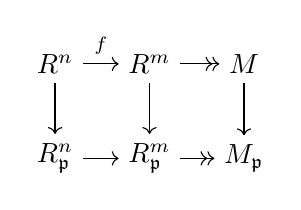
\begin{tikzpicture}[auto]
  \node (Rn) at (0, 1.2) {$R^n$}; \node (Rm) at (1.2, 1.2) {$R^m$};\node (M) at (2.4, 1.2) {$M$};
  \node (Rpn) at (0, 0) {$R_{\mathfrak{p}}^n$};   \node (Rpm) at (1.2, 0) {$R_{\mathfrak{p}}^m$};\node (Mp) at (2.4, 0) {$M_{\mathfrak{p}}$};
  \draw[->] (Rn) to node {$\scriptstyle f$} (Rm);\draw[->>] (Rm) to node {} (M);
  \draw[->](Rn) to node {} (Rpn);\draw[->](Rm) to node {} (Rpm);\draw[->](M) to node {} (Mp);
  \draw[->] (Rpn) to node {} (Rpm);\draw[->>] (Rpm) to node {} (Mp);
\end{tikzpicture}

Poitou-Tateを計算していきたい.


\begin{thebibliography}{a99}

\bibitem[Bourbaki]{} Bourbaki,N., $\mathrm{\acute{E}}$l$\mathrm{\acute{e}}$ments de Math$\mathrm{\acute{e}}$matique, Alg$\mathrm{\grave{e}}$bre Commutative, Chap. 7, Hermann, Paris (1965).

   \bibitem[de Shalit]{de Shalit}  de Shalit,E., Iwasawa Theory of Elliptic Curves with Complex Multiplication. Perspectives in Mathematics, vol. 3, Academic Press, Boston,(1987).

    \bibitem[Johnson Kings]{JK} Johnson,L.J., ; Kings,G., On the equivariant main conjecture for imaginary quadratic fields.
J. Reine Angew. Math. 653 (2011), 75-114.

\bibitem[Kurihara]{Kurihara} Kurihara,M., Iwasawa theory and Fitting ideals, J. reine angew. Math. 561 (2003), 39-86.



  \bibitem[Milne 1]{M1} Milne,J.S., Arithmetic duality theorems, volume 1 of Perspectives in Mathematics.
Academic Press Inc., Boston, MA, (1986)

  \bibitem[Milne 2]{Milne 2} Milne,J.S., Lectures on Etale Cohomology, available at www.milne.org, (1998).

\bibitem[Northcott]{Nor} Northcott,D.G., Finite free resolutions, Cambridge Univ. Press (1976).

    \bibitem[Rubin 1]{Rubin} Rubin,K., The  "main conjectures"  of Iwasawa theory for imaginary quadratic fields, Invent.
math. 103 (1991), 25-68.

  \bibitem[Rubin 2]{Rubin 2} Rubin,K., More  "main conjectures" for imaginary quadratic fields, Elliptic curves and related
topics,CRMProc. Lect. Notes 4, Amer. Math. Soc., Providence, RI (1994), 23-28.

  \bibitem[Rubin 3]{Rubin 3} Rubin,K., Euler systems, Annals of Math. Studies 147, Princeton Univ. Press (2000).

  \bibitem[Tate]{Tate} Tate,J., Duality theorems in Galois cohomology over number fields.  Proc. Internat.
Congr. Mathematicians,  Inst. Mittag-Leffler, Djursholm, (1962),288-295.
  \bibitem[Washington]{Washington} Washington,L., Introduction to Cyclotomic Fields, 2nd edition, Graduate Texts in Math. 83, Springer-Verlag (1997)
\end{thebibliography}

\end{document}
